%%%%%%%%%%%%%%%%%%%%%%%%%%% asme2ej.tex %%%%%%%%%%%%%%%%%%%%%%%%%%%%%%%
% Template for producing ASME-format journal articles using LaTeX    %
% Written by   Harry H. Cheng, Professor and Director                %
%              Integration Engineering Laboratory                    %
%              Department of Mechanical and Aeronautical Engineering %
%              University of California                              %
%              Davis, CA 95616                                       %
%              Tel: (530) 752-5020 (office)                          %
%                   (530) 752-1028 (lab)                             %
%              Fax: (530) 752-4158                                   %
%              Email: hhcheng@ucdavis.edu                            %
%              WWW:   http://iel.ucdavis.edu/people/cheng.html       %
%              May 7, 1994                                           %
% Modified: February 16, 2001 by Harry H. Cheng                      %
% Modified: January  01, 2003 by Geoffrey R. Shiflett                %
% Use at your own risk, send complaints to /dev/null                 %
%%%%%%%%%%%%%%%%%%%%%%%%%%%%%%%%%%%%%%%%%%%%%%%%%%%%%%%%%%%%%%%%%%%%%%

%%% use twocolumn and 10pt options with the asme2ej format
\documentclass[twocolumn,10pt]{asme2ej}

\usepackage{graphicx} %% for loading jpg figures
\usepackage{tabu}
\usepackage{float}
\usepackage{tabularx}
\usepackage{subfigure}
\usepackage{amsmath}
\usepackage{multicol}
\usepackage{color,soul}
\usepackage{xcolor}

\newcommand{\highlight}[1]{%
  \colorbox{yellow!}{$\displaystyle#1$}}
%% The class has several options
%  onecolumn/twocolumn - format for one or two columns per page
%  10pt/11pt/12pt - use 10, 11, or 12 point font
%  oneside/twoside - format for oneside/twosided printing
%  final/draft - format for final/draft copy
%  cleanfoot - take out copyright info in footer leave page number
%  cleanhead - take out the conference banner on the title page
%  titlepage/notitlepage - put in titlepage or leave out titlepage
%  
%% The default is oneside, onecolumn, 10pt, final


\title{Application of computational fluid dynamics and process modelling to investigate low-load operation of a subcritical utility-scale boiler.}

%%% first author
\author{Brad T. Rawlins\thanks{Corresponding author}
    \affiliation{
	Ph.D. Candidate\\
	Department of Mechanical \\Engineering\\
	University of Cape Town\\
    Email: rwlbra001@myuct.ac.za
    \vspace{5mm}
    }	
    
}

%%% second author
%%% remove the following entry for single author papers
%%% add more entries for additional authors
\author{Ryno Laubscher 
    \affiliation{Associate Professor\\
    Department of Mechanical \\Engineering\\
	Stellenbosch University\\
    Email: rlaubscher@sun.ac.za
    }
}

%%% third author
%%% remove the following entry for single author papers
%%% add more entries for additional authors
\author{Pieter Rousseau
    \affiliation{Professor\\
        Department of Mechanical \\Engineering\\
        University of Cape Town\\
        Email: pieter.rousseau@uct.ac.za
    }
}


\begin{document}

\maketitle    

%%%%%%%%%%%%%%%%%%%%%%%%%%%%%%%%%%%%%%%%%%%%%%%%%%%%%%%%%%%%%%%%%%%%%%
\begin{abstract}
{\it To enable the inclusion of intermittent renewable energy sources on existing power grids requires base-load coal-fired power plants to operate flexibly, including fast load changes and continuous low-load operation. Low-load operation of a 620 $MWe$ sub-critical boiler is analysed with the aid of a co-simulation methodology that incorporates a detail three dimensional computational fluid dynamics (CFD) model together with a one dimensional process model. A discretized one dimensional model of the water/steam circuit was developed for the furnace, the radiant superheaters and the convective/back pass heat exchangers. This is coupled with a detailed CFD model incorporating the furnace and radiant superheaters using a Eulerian-Eulerian reference frame. The coupled model is used to investigate the combustion stability, water/steam side effects, and the radiant heat exchanger operational limits for six different burner firing arrangements at a low boiler load of 32\% of Maximum Continuous Rating. The results show that certain firing arrangements can lead to a high risk of fire-side corrosion and overheating of heat exchanger components. Based on analyses of combustion stability, boiler efficiency and the safe operation of heat exchanger components, a mixed firing arrangement with a higher secondary air mass flowrate for non-firing burners was selected as the best operational strategy at this low load for the boiler under investigation.
}
\end{abstract}

%%%%%%%%%%%%%%%%%%%%%%%%%%%%%%%%%%%%%%%%%%%%%%%%%%%%%%%%%%%%%%%%%%%%%%
\begin{nomenclature}
\entry{}{\textit{Variables}}
\entry{$A$}{Area [$m^2$]}
\entry{$A_p$}{Particle surface area [$m^2$]}
\entry{$A_{pn}$}{Projected particle surface area [$m^2$]}
\entry{$A_{c}$}{Carbon pre-exponential factor [$s^{-1}$]}
\entry{$A_{vol}$}{Volatile pre-exponential factor [$s^{-1}$]}
\entry{$d_p$}{Particle diameter [$m$]}
\entry{$E$}{Fluid total energy [$J/kg$]}
\entry{$E_{a,c}$}{Carbon activation energy [$J/kmol$]}
\entry{$E_{a,vol}$}{Volatile activation energy [$J/kmol$]}
\entry{$E_p$}{Particle emission power [$W/m^3$]}
\entry{$f_{heat}$}{Near surface char oxidation fraction [$-$]}
\entry{$f_{p}$}{Forward scattering factor [$-$]}
\entry{$G$}{Incident radiation [$W/m^2$]}
\entry{$g$}{Gravitational constant [$m/s^2$]}
\entry{$h_{fg}$}{Enthalpy of evaporation [$J/kg$]}
\entry{$h_M$}{Mixture enthalpy [$J/kg$]}
\entry{$h_{rxn}$}{Enthalpy of reaction [$J/kg$]}
\entry{$J_k$ }{Species diffusion flux [$m^2/s$]}
\entry{$m_{0,vol}$}{Original mass of volatiles [$kg$]}
\entry{$m_{char}$}{Mass of carbon [$kg$]}
\entry{$m_{evap}$}{Mass of moisture [$kg$]}
\entry{$m_{vol}$}{Mass of volatiles [$kg$]}
\entry{$N_{p}$}{Number of particles [$-$]}
\entry{$P$}{Perimeter [$m$]}
\entry{$p$}{Pressure [$Pa$]}
\entry{$p_{O_{2}}$}{Partial pressure of $O_2$ [$Pa$]}
\entry{$\dot{Q}_{conv}$}{Convective heat transfer rate [$W$]}
\entry{$\dot{Q}_{rad}$}{Radiative heat transfer rate [$W$]}
\entry{$\dot{Q}_{w}$}{Wall heat transfer rate [$W$]}
\entry{$R$}{Universal gas constant [$J/molK$]}
\entry{$R_{c}$}{Carbon reaction rate [$s^{-1}$]}
\entry{$R_{diff}$}{Diffusion reaction rate [$s^{-1}$]}
\entry{$R_{vol}$}{Volatile reaction rate [$s^{-1}$]}
\entry{$S$}{\hl{Mass source term}[$kg/m^3$]}
\entry{$S_m$}{\hl{Momentum source term} [$/m^3$]}
\entry{$S_h$}{\hl{Energy source term} [$W/m^3$]}
\entry{$S_k$}{\hl{Species source term} [$kg/m^3$]}
\entry{$T_g$}{Gas temperature [$K$]}
\entry{$T_p$}{Particle temperature [$K$]}
\entry{$t$}{Time [$s$]}
\entry{$u$}{Velocity [$m/s$]}
\entry{$V$}{Volume [$m^3$]}
\entry{$Y_k$}{Species mass fraction [$kg/kg$]}
\entry{$x$}{Quality [$-$]}
\entry{}{\textit{Greek Variables}}
\entry{$\alpha_g$}{Gas absorption coefficient [$m^{-1}$]}
\entry{$\alpha_H$}{Mixture void fraction [$-$]}
\entry{$\alpha_p$}{Particle absorption coefficient [$m^{-1}$]}
\entry{$\epsilon_p$}{Particle emissivity [$-$]}
\entry{$\rho$}{Gas density [$kg/m^3$]}
\entry{$\rho_{eff}$}{Effective density [$kg/m^3$]}
\entry{$\rho_g$}{Gas density [$kg/m^3$]}
\entry{$\rho_l$}{Liquid density [$kg/m^3$]}
\entry{$\rho_M$}{Mixture density [$kg/m^3$]}
\entry{$\rho_p$}{Particle density [$kg/m^3$]}
\entry{$\sigma_{SB}$}{Stefan-Boltzmann constant [$W/m^2K^4$]}
\entry{$\sigma_{p}$}{Particle scattering coefficient [$m^{-1}$]}
\entry{$\phi$}{Scalar variable [$-$]}
\entry{}{\textit{Abbreviations}}
\entry{$MCR$}{Maximum continuous rating}
\entry{$CFPP$}{Coal fired power plant}
\entry{$CFD$}{Computational fluid dynamics}
\entry{$SH$}{Superheater}
\entry{$EE$}{Eulerian-Eulerian}
\entry{$WSGGM$}{Weighted sum of gray gas model}
\entry{$RTE$}{Radiative transport equation}
\entry{$HHV$}{Higher heating value}
\entry{$DAF$}{Dry ash free}
\entry{$AR$}{As-received}
\entry{$PA$}{Primary air}
\entry{$SA-AH$}{Secondary air - air heater}
\entry{$SA$}{Secondary air}
\entry{$RH$}{Reheater}
\entry{$ATT$}{Attemperator}
\entry{$EC$}{Economiser}
\end{nomenclature}
%%%%%%%%%%%%%%%%%%%%%%%%%%%%%%%%%%%%%%%%%%%%%%%%%%%%%%%%%%%%%%%%%%%%%%
\section{Introduction}
The use of coal-fired power plants (CFPP) for electricity generation is intended to be phased out to reduce the rate of climate change. However, the move to sustainable generation sources poses great challenges for developing countries due to the long transition times and costs involved \cite{ugum2019}. Due to the abundance of coal resources present in Southern Africa, CFPPs are still the dominant power generation source, with approximately 80\% of the energy needs being met using CFPPs \cite{eskom}.\\

The integration of renewable energy sources will push CFPPs from primarily base load operation to a mid-merit/flexible operating protocol, which includes prolonged operation at low-loads. Long term deviation from design conditions can lead to operational inefficiencies affecting combustion stability \cite{Hernik2020}, an increase in harmful emissions \cite{Chang2021}, and the localised overheating of heat exchangers due to insufficient cooling being provided by the internal working fluid \cite{Modlinski2019}.\\

While full scale testing or experimentation on CFPPs is deemed too expensive to pursue, mathematical models that can accurately capture the thermal response of boilers at varying loads can be used to determine the safe and efficient operating limits \cite{Laubscher2019b}. Computational fluid dynamics (CFD) allows for the modelling of full-scale CFPP boilers, at steady-state operating conditions. CFD simulations have been successfully used to model a variety of CFPP boiler types (\cite{Laubscher2019a}, \cite{Gu2020}) and cover various aspects such as pollution control (\cite{Du2017},\cite{Fan2001}), gas-solid flow effects (\cite{Chen2017}) and boiler retrofitting (\cite{Gu2020}, \cite{He2007}).\\

Recent CFD studies investigating low-load operation of CFPP boilers have focused on the combustion stability, harmful emissions and the gas flow-solid flow interactions \cite{Jiang2021}. The works of Belosevic et al \cite{Belosevic2019a} found that the low-load operation of boilers considerably affects the flow and temperature fields, the flame geometry, chemical reactions and concentrations of combustion products.\\

Hernik et al \cite{Hernik2020} investigated the effects of using different mill system configurations at a minimum boiler load of 40\%. The most favourable mill system configuration was selected based on the case that exhibited suitable combustion stability and emission of harmful substances. Similarly, Chang et al \cite{Chang2021} investigated the various firing arrangements of a 630 $MWe$ tangentially fired boiler. A burner angle of -15 $^\circ$ was found to be the optimal arrangement resulting in the best compromise between combustion stability and lower emissions. The aforementioned research specifically investigated combustion and gas-side effects.\\

Various one-dimensional (1-D) process modelling approaches have also been used by researchers to investigate the water and gas side heat transfer interactions. These studies are usually aimed at investigating a transient event, such as a sudden disturbance, start-up, or boiler load ramping \cite{Alobaid2017}. Due to the non-uniformities found in CFPP furnaces which are composed of complex combustion dynamics, gas-solid interactions and  radiation heat transfer phenomena, 1-D process models can not resolve the fireside with sufficient accuracy. However it can adequately resolve the waterside energy and momentum transport in a computationally inexpensive manner.\\
\newpage
The use of coupled simulations has proven to solve the deficiencies of a full 1-D process model by coupling the fireside CFD results to a 1-D water side model. Laubscher and Rousseau \cite{Laubscher2020} conducted a comprehensive numerical study on the impact of particle radiation properties for high ash coals using ANSYS Fluent v19.2\textsuperscript{\textregistered} and Flownex SE\textsuperscript{\textregistered}, while Yu et al \cite{Yu2019} used a coupled simulation methodology to estimate the superheater (SH) metal temperatures of a 660 $MWe$ tangentially-fired coal boiler.\\

However, to the authors’ knowledge, the integration of a 1-D process model with a detail CFD model has not been used to investigate the steam side operational performance of a CFPP boiler specifically at low-load. The goal of the current work is therefore to investigate the effect of burner firing configuration on various process parameters such as steam temperatures, spray water flowrates and metal temperatures at low-load, using a detailed CFD model on the gas side coupled to a comprehensive process model on the water/steam side.\\

To establish the accuracy of the CFD modelling approach a validation study was first conducted at loads of 100\%, 80\% and 60\% Maximum Continuous Rating (MCR) and compared to actual plant measurements. Thereafter the model was applied to simulate the boiler operation at 32\% of MCR with six different firing configurations.

\section{Mathematical model}
\subsection{Computational fluid dynamics modelling}
\subsubsection{Fluid flow, turbulence and combustion modelling}
The flue gas-side was modelled using a Eulerian framework. The species transport modelling approach was used to approximate the mixture of chemical species in the gas phase. This approach solves a species continuity equation for each constituent present in the mixture. To reduce the computational burden, it was assumed that the various processes were in steady-state. \hl{The governing equations for the gas phase are written below in their respective Reynolds averaged forms}.\\
Mass conservation:
\begin{equation}\label{eqn_RANS_mass}
\frac{\partial}{\partial x_{i}}(\rho \bar{u}_{i})=\highlight{S}
\end{equation}
Momentum conservation:
\begin{equation}\label{eqn_momentum}
\begin{split}
&\frac{\partial}{\partial x_{i}}(\rho_{eff} u_{i}u_{j})+\frac{\partial \overline{p}}{\partial x_{j}}=\frac{\partial}{\partial x_{i}}\left[\mu\left\{\frac{\partial u_{j}}{\partial x_{i}}+\frac{\partial u_{i}}{\partial x_{j}}-\frac{2}{3}\delta_{ij}\frac{\partial u_{i}}{\partial x_{i}}\right\}\right]+\\
&\frac{\partial}{\partial x_{i}}(-\rho\overline{u_{i}^{'}u_{j}^{'}})+S_m
\end{split}
\end{equation}
Energy conservation:
\begin{equation}\label{eqn_energy}
\frac{\partial }{\partial x_{i}} (u_{i}[\rho E+p])=\frac{\partial }{\partial x_{j}}\left[\lambda\frac{\partial T_{g}}{\partial x_{j}}\right] +S_{h}
\end{equation}
Species transport:
\begin{equation}\label{eqn_species}
\begin{split}
&\frac{\partial}{\partial x_{i}}(\rho u_{j}Y_{k})=-\frac{\partial}{\partial x_{j}}(\vec{J_{k}})+ \sum_r R_{j,r} + S_{k}\\
&k = 1,2,3...N
\end{split}
\end{equation}

To correctly account for the particle inertial effects on the gas phase convection, the model makes use of an effective density which is defined as follows:
\begin{equation} \label{eqn_eff_rho}
	\rho_{eff} = \frac{\rho \rho_p \left( \phi_{mp} + 1 \right)}{\rho \phi_{mp} + \rho_p}
\end{equation}

In the present study the realizable k-$\varepsilon$ turbulence model was utilized to address the turbulence closure problem. This model has been successfully used by researchers (\cite{Belosevic2019a},\cite{Laubscher2019a} and \cite{Modlinski2019}), in modelling the effects of coal-fired swirl burners. The model generally produces higher accuracy results, when compared to the standard k-$\varepsilon$ model, for problems incorporating swirling and separating flows.\\

The process of coal combustion comprises of four sequential steps namely, inert heating and evaporation of moisture, devolatilization, char oxidation and gas phase reactions. Equations (\ref{eqn_vol_rate}) and (\ref{eqn_vol_arrhenuis}) show the single rate kinetic model utilized in this study, to model the devolatilization process.
\begin{gather}
\frac{dm_{vol}}{dt} = R_{vol}(m_{0,vol}-m_{vol}) \label{eqn_vol_rate} \\
\begin{split}
&R_{vol} = A_{vol}exp\left(\frac{E_{a,vol}}{RT_p}\right)\\
&A_{vol} = 2\times10^5 [s^{-1}]\,\,\,\,\,\,\,\,\,\,E_{a,vol} = 6.7\times10^7 [J/kmol] \label{eqn_vol_arrhenuis}
\end{split}
\end{gather}

A devolatilization temperature of 553 [$K$] \cite{Ranade2015} along with the kinetic parameters (Eqn. \ref{eqn_vol_arrhenuis}) of Sheng et al \cite{Sheng2004} were utilized in the present study.\\
\newpage
The char oxidation process is modelled using the diffusion-kinetics limited model developed by Baum and Street \cite{Baum1971}, which is given in Eqn. (\ref{eqn_char_rate}). The product species of the char oxidation reaction was set to $CO$ as shown in Eqn. (\ref{eqn_CO_reaction}). 
\begin{gather}
\frac{dm_{char}}{dt} = -A_p p_{O_{2}} \frac{R_{diff}R_c}{R_{diff} + R_c}  \label{eqn_char_rate}\\
C_{(s)}+0.5O_{2(g)}\to CO_{(g)} \label{eqn_CO_reaction}
\end{gather}
The diffusion and kinetic rates of Eqn. (\ref{eqn_char_rate}) are defined in Eqn. (\ref{eqn_char_diff_rate})  and Eqn. (\ref{eqn_char_kin_rate}) with the kinetic parameters again taken from the works of Sheng et al \cite{Sheng2004}.
\begin{gather}
R_{diff} = \frac{5\times10^{-12}}{d_p} \left(\frac{T_g+T_p}{2}\right)^{0.75} \label{eqn_char_diff_rate}\\
\begin{split}
&R_{c} = A_{c}exp\left(\frac{E_{a,c}}{RT_p}\right)\\
&A_{c} = 0.0053 [kg/m^2sPa]\,\,\,\,\,\,\,\,\,\,E_{a,c} = 8.37\times10^7 [J/kmol]
\end{split}
 \label{eqn_char_kin_rate}
\end{gather}

The turbulence-chemistry interactions of the gas phase reactions were approximated using the eddy-dissipation-finite rate model used in ANSYS Fluent v19.5\textsuperscript{\textregistered} which calculates three rates, namely chemical reaction rate, turbulent production eddies dissipation rate and reaction eddies dissipation rate. It then applies the minimum of the three for the source terms calculations. A description of the CFD gas phase reactions of the boiler under consideration, using the same coal, was previously published in the works of Laubscher and Rousseau \cite{Laubscher2019b}.

\subsubsection{Particle modelling}
The particles are modelled using a Eulerian reference frame, similar to the studies of Knaus et al \cite{Knaus2001a} and Benim et al \cite{Benim2005}. Both successfully used a Eulerian-Eulerain (EE) model to capture the characteristics of coal combustion and furnace heat transfer with adequate accuracy. The pseudo particle mass concentrations transported into the domain are modelled using the general scalar field transport equation with the necessary modifications to account for heat and mass transport \cite{Versteeg2007}. The pseudo-particles scalar fields are used to define the fuel characteristics based on the proximate analysis composition, namely consisting of moisture, volatile matter, fixed carbon and ash. The scalar field equations are provided in Tab. \ref{tab_scalars}.\\

\begin{table}[h!]
\centering
\caption{Scalar field equation descriptions}\label{tab_scalars}  
\vspace{2mm}     
\begin{tabularx}{3.25in}{p{0.4in} p{1.25in} l}
\hline
Variable &Description& Transport equation \\
\hline
$\phi_{mp0}$ &Original/initial mass of particles& $\frac{\partial}{\partial x_{i}}(\rho u_{i} \phi_{mp0})=0$\\
$\phi_{M}$&Moisture present in particles&$\frac{\partial}{\partial x_{i}}(\rho u_{i} \phi_{M})=\frac{1}{V} \frac{dm_{evap}}{dt}$\\
$\phi_{VM}$&Volatile matter present in particles&  $\frac{\partial}{\partial x_{i}}(\rho u_{i} \phi_{VM})=\frac{1}{V}\frac{dm_{vol}}{dt}$\\
$\phi_{FC}$&Fixed carbon present in particles&$\frac{\partial}{\partial x_{i}}(\rho u_{i} \phi_{FC})=\frac{1}{V}\frac{dm_c}{dt}$\\
$\phi_{ASH}$&Ash present in particles&$\frac{\partial}{\partial x_{i}}(\rho u_{i} \phi_{ASH})=0$\\
$\phi_{hp}$&Enthalpy of particle&Equation \eqref{eqn_phi_hp}\\
\hline
\end{tabularx}
\end{table}

The energy transport of the pseudo particle phase, is captured by defining a particle phase energy balance equation, which in turn uses the particle enthalpy.
\begin{equation}\label{eqn_phi_hp}
\frac{\partial}{\partial x_{i}}( \rho u_{i} \phi_{hp} )=\left( f_{heat}\frac{dm_{c}}{dt}h_{rxn} + \dot{Q}_{rad} + \dot{Q}_{conv} - \frac{dm_{evap}}{dt}h_{fg} \right) \frac{1}{V} 
\end{equation}

The equation accounts for all the processes associated with energy transport to the particle, namely convection $\left(\dot{Q}_{conv}\right)$, radiation $\left(\dot{Q}_{rad}\right)$, latent heat transport $\left(\frac{dm_{evap}}{dt}h_{fg}\right)$ and near surface char oxidation $\left(f_{heat}\frac{dm_{c}}{dt}h_{rxn}\right)$. This gives the model the ability to track the particle temperature in the domain, which distinguishes it from the thermal equilibrium approach incorporated by previous studies using an EE approach (\cite{Benim2005}, \cite{Vicente2003} and \cite{Cai2015}). The particle temperature is important in describing the sequential steps found in modelling combustion processes, especially at low boiler loads where mixing and ignition become problematic. \hl{To solve the additional transport equations and their source terms user defined functions, utilized by ANSYS Fluent, were developed using the C programming language.}

\subsection{Heat transfer modelling}
Radiation heat transfer is the dominant form of heat transfer found in industrial furnaces \cite{Basu2000} and is solved by applying the gray-participating-gas and particle medium configuration of the radiation transport equation (RTE) \cite{Modest2013} shown in Eqn. (\ref{eqn_RTE}).
\begin{equation}\label{eqn_RTE}
\begin{split}
&\frac{d I(\vec{r},\hat{s})}{ds} = \alpha_g \frac{\sigma_{SB} T_{g}^4}{\pi}-(\alpha_g+\alpha_p+\sigma_p)I(\vec{r},\hat{s}) + \\
&\frac{\sigma_p}{4\pi}\int_{4\pi}I(\vec{r},\hat{s})\Phi d \Omega
\end{split}
\end{equation}
In the present work the RTE is solved using the P1 model. Ranade and Gupta \cite{Ranade2015} illustrated minimal differences between the two common radiation models (namely the P1 and discrete ordinates (DO)) for the resultant wall heat transfer rate values when modelling a 210 $MWe$ CFPP boiler. The P1 radiation model can include the effects of particle absorption ($\alpha_p$) and scattering ($\sigma_p$) as well as gas mixture absorption ($\alpha_g$). The P1 model transport variable is the incident radiation flux (G), and can be written for a particle laden domain as:
\begin{equation}
\begin{split}
&\frac{\partial}{\partial x_{i}}\left(\Gamma\frac{\partial G}{\partial x_{i}}\right)=\left(\alpha_g+\alpha_p\right)G-4\left(\alpha_g \sigma_{SB} T_{g}^4-\pi E_p \right)\\
&\Gamma = \frac{1}{\alpha_g+\alpha_p+\sigma_p}
\end{split}
\end{equation}

The flue gas absorptivity was calculated using the domain based weighted sum of gray gas model (WSGGM) using the coefficients determined by Smith et al \cite{Smith1982}. The WSGGM accounts for the radiation emitted by tri-atomic gases, namely $CO_2$, $H_2O$ and $SO_2$ present in the flue gas stream. The Eulerian description of the terms $\alpha_p$, $\sigma_p$ and $E_b$ are determined using the effective number of particles ($N_p = \rho \phi_{mp0} V / \left( \rho_p \pi \bar{d_p}^3 /6 \right)$) present in a cell. The equations for the radiative properties are given in Eqn. (\ref{eqn_part_abs}) through Eqn. (\ref{eqn_part_emisp}).
\begin{gather}
\alpha_p = \frac{\epsilon_p A_{pn}N_p}{V} \label{eqn_part_abs}\\
\sigma_p = \frac{(1-\epsilon_p)(1-f_p) A_{pn}N_p}{V} \label{eqn_part_scat} \\
E_p = \frac{\epsilon_p \sigma_{SB} T_p^4 A_{pn}N_p}{V}\label{eqn_part_emisp}
\end{gather}

It is important to note that variable properties for ($\epsilon_p$) and ($f_p$) were used, that are based on the correlations of Lockwood et al \cite{Lockwood1986} and Yin \cite{Yin2015} respectively.
\begin{figure*} 
\centerline{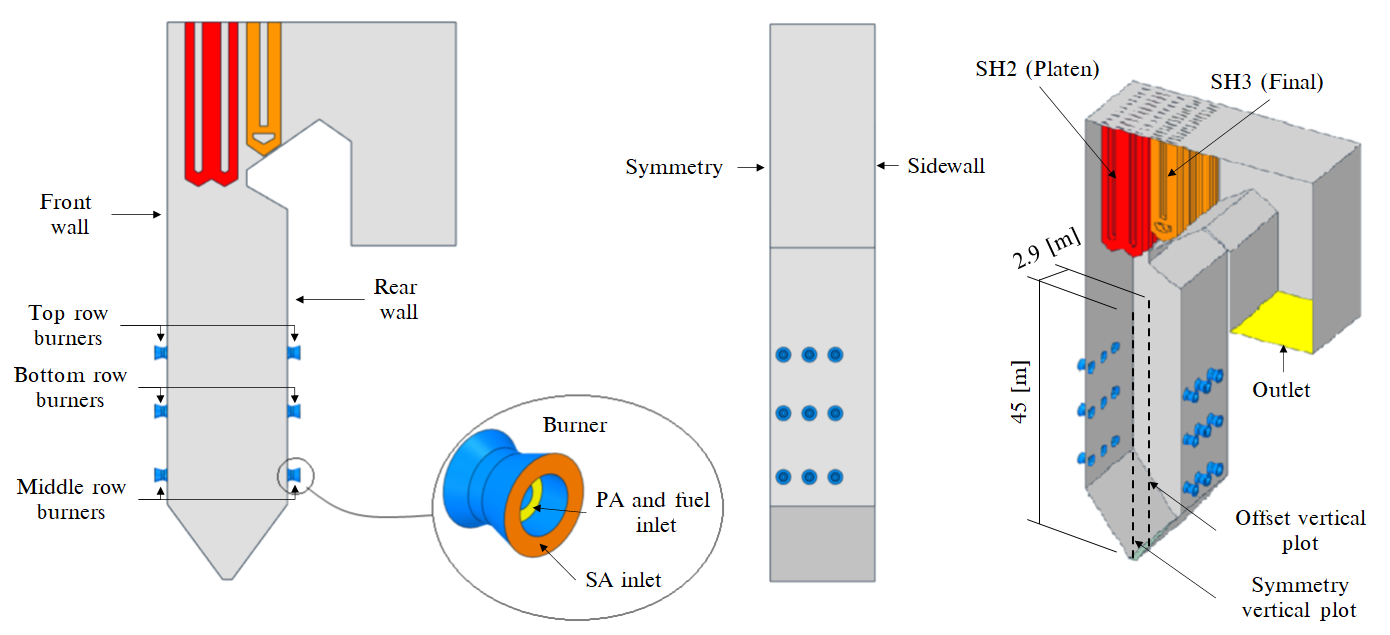
\includegraphics[scale=0.45]{GEOMETRY}}
\caption{Boiler geometry and layout}
\label{fig_geometry}
\end{figure*}
\begin{figure*}[h!]
\centering
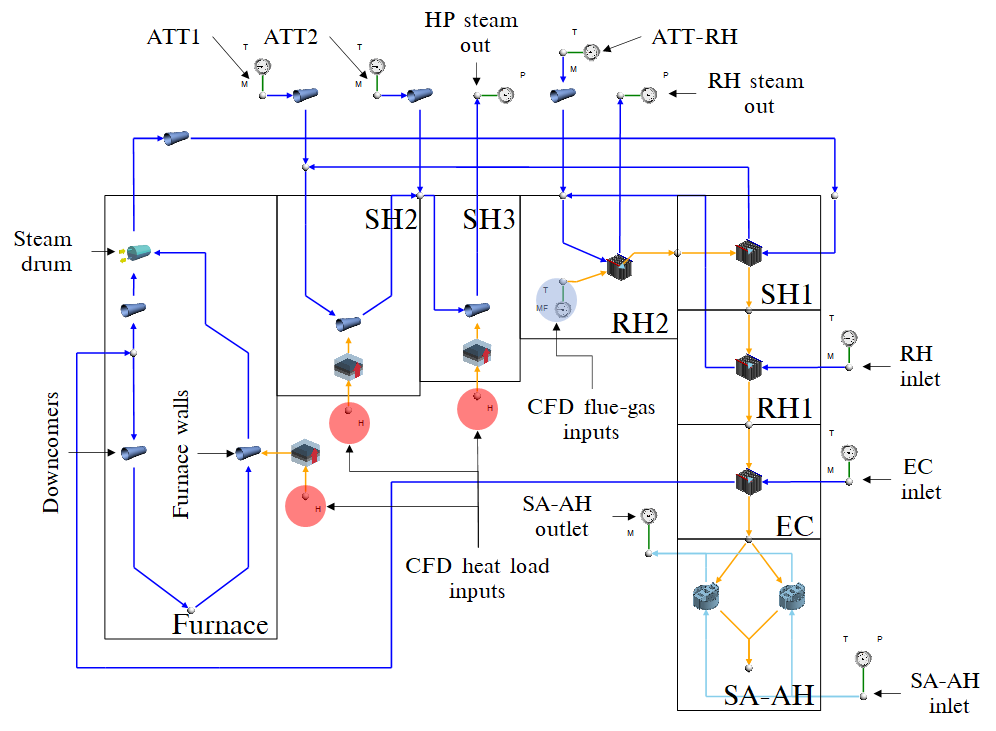
\includegraphics[scale=0.5]{FLOWNEX_SETUP}
\caption{Process model of boiler set-up including the downstream convective components using Flownex SE 2021}
\label{fig_flownex}
\end{figure*}
\subsection{Process simulation model}
A 1D discretized model of the furnace evaporator, platen SH, final SH, and subsequent downstream heat exchangers was developed using Flownex SE\textsuperscript{\textregistered} 2021. \hl{The coupling of the two models makes use of a decoupled approach, where the CFD simulation data is exchanged to the Flownex model when convergence of each case is achieved, a further explanation of the coupling interface is given in Section} \ref{sec_set_up}. The model simulates the internal convection heat transfer inside the tubes and the conduction through the tube walls. The model is able to simulate the attemperation flows and momentum transport through the steam/water circuit. The heat exchangers were modelled using a homogeneous two-phase mixture approach, which assumes that the fluid properties, phase velocities and temperatures are uniform per cross-sectional area. The homogeneous mixture fraction and mixture density are defined in Eqn. (\ref{eqn_vol_frac}) and Eqn. (\ref{eqn_mix_rho}) respectively.
\begin{gather}
\alpha_H = \frac{\rho_l x}{\rho_lx + \rho_g(1-x)} \label{eqn_vol_frac}\\  
\rho_M = (1-\alpha_H)\rho_l + \alpha_H\rho_g \label{eqn_mix_rho}
\end{gather}
Applying the mixture density the following transport equations are solved per process model component;

\begin{equation}\label{eqn_mix_conti}
\frac{\partial}{\partial t}(\rho_M A)+\frac{\partial}{\partial s}(\rho_MAu) = 0
\end{equation}
\begin{equation}\label{eqn_mix_mom}
\frac{1}{A} \frac{\partial}{\partial t}(\rho_M A u)+\frac{1}{A} \frac{\partial}{\partial s}(\rho_M A u^2) = -\frac{\partial p}{\partial s}-\frac{\tau_W P}{A}- \rho_M g \frac{\partial z}{\partial s}
\end{equation}
\begin{equation}\label{eqn_mix_energy}
\begin{split}
&\frac{\partial}{\partial t}(\rho_Mh_M)+\frac{1}{A}\frac{\partial}{\partial s}(\rho_MAuh_M)+\frac{1}{2}\frac{\partial}{\partial s}(\rho_Mu^2)+\\
&\frac{1}{2A}\frac{\partial}{\partial s}(\rho_MAu^3)=\frac{\partial p}{\partial t} + \frac{\dot{Q}_w}{V}-g\rho_Mu\frac{\partial z}{\partial s}
\end{split}
\end{equation}

The process model is used to determine the required attemperation flow rates to achieve the exit steam conditions, boiler efficiency, and steam generation for each case. The results of this model aid in determining the best firing combination of burner rows for continuous low-load operation, and the effects on the water-side of the boiler system.

\section{Case study boiler description \& set-up}
In this section the numerical model configuration, for both the CFD and process model, will be explained, covering the boiler geometry, the process model set-up, the various  modelling inputs (i.e. fuel characteristics and boundary conditions) and the numerical solution strategy.

\subsection{Geometry \& process model set-up} \label{sec_set_up}
The modelled  boiler is a two-pass sub-critical power boiler with a furnace depth of 13.77 [$m$], width of 14.01 [$m$] and height of 64 [$m$]. The CFD geometric model (of Fig. \ref{fig_geometry}) makes use of a symmetry plane at half the width of the furnace. This was done to reduce the cell count of the numerical mesh. Both the platen and final SH are modelled as solid wall panels, with transverse pitches of 1.143 [$m$] and 0.8 [$m$] respectively. There are three levels of burners located on both the front and rear walls at heights of 11.9 [$m$], 19.3 [$m$] and 26 [$m$]. Figure \ref{fig_geometry} shows the modelled half of the furnace along with the locations of the platen SH, final SH, boundary walls (front, rear and side) and the domain outlet and inlets.\\

The boiler furnace is fed by six mills, each supplying pulverised fuel and primary air (PA) mixture to a burner row consisting of six \hl{swirl} burners. This mixture is injected through the inner burner annulus while the secondary air (SA) is fed through the outer annulus as seen Fig. \ref{fig_geometry}.\\ 

\hl{The CFD wall boundary conditions were modelled using ANSYS Fluent's convection boundary condition type. This boundary condition requires internal free stream temperature (water or steam) and the inside heat transfer coefficient. To determine these values a 0D process model was set-up using the Gurwich approach to estimate the internal heat transfer coefficient and internal temperature for these load cases.}\\

The process model of the boiler configuration is shown in Fig. \ref{fig_flownex}. The process model includes all the heat exchangers up to and downstream of the final SH, which include the secondary reheater (RH2), primary SH (SH1), primary reheater (RH1), economiser (EC) and the SA air heaters (SA-AH). The model includes all the relevant attemperators (ATT1, ATT2 and ATT-RH), inlets and outlets. The process model is used to determine the required attemperation flowrates and water/steam side thermal response. The furnace water-walls are represented by a single lumped pipe flow component and forms part of the natural circulation system that includes the downcomers and steam drum. As with the furnace walls, the platen and final SHs are similarly represented by a single lumped parameter pipe flow component, interconnected with nodes that introduce the attemperation flows to the water/steam side.\\ 

The coupling interface between the simulation models are the heat-exchanger external tube surfaces, namely the furnace, platen and final SH walls. The CFD heat loads are used as energy sources for these components as indicated in Fig. \ref{fig_flownex}. The furnace heat load to the evaporator walls determines the circulation rate through the evaporator. The steam drum separates the gas from the liquid, with the liquid water being recirculated through the evaporator and the saturated vapour (steam) being sent through the main steam line for superheating. Thus the steam generation is calculated. Furthermore, the CFD flue-gas results (i.e. composition, mass flow and temperature) exiting the final SH are used as boundary values for the heat exchangers downstream of the final SH (SH3), as shown in Fig. \ref{fig_flownex}. The steam flow boundary values for the RH and EC sections are fixed inlet mass flows and temperatures with the corresponding outlets set to a fixed pressure.\\

Figure \ref{fig_heat_exchanger_model} illustrates the heat exchanger component process model. This component is used for the heat exchangers downstream of SH3 (refer to Fig. \ref{fig_flownex}).\\

The component model accounts for the radiative (gas and direct), convective and conduction heat transfer mechanisms to and from the gas-side and steam-side control volumes, as well as between up- and downstream heat exchangers on the gas side. The total heat transferred to the water-side control volume can be written as the sum of the absorbed direct radiation and the combined convective and gas radiative heat transfer (i.e. $\dot{Q}_{steam}=\dot{Q}_{abs}+\dot{Q}_{cr}$). The external heat transfer coefficient, from the flue-gas to the heat-exchanger walls makes use of the Gnielinski correlation \cite{Gnielinski2016} for the various heat-exchanger tube arrangements. Figure \ref{fig_heat_exchanger_model} incorporates the direct radiative interactions in each heat-exchanger. It shows that the portion of direct radiation from the preceding heat exchanger that is not absorbed is joined by the bypass radiation ($\dot{Q}_{bypass}$) of the flue-gas control volume which together make up  the direct radiation passed on to the downstream components.
\begin{figure*}[h!]
\centerline{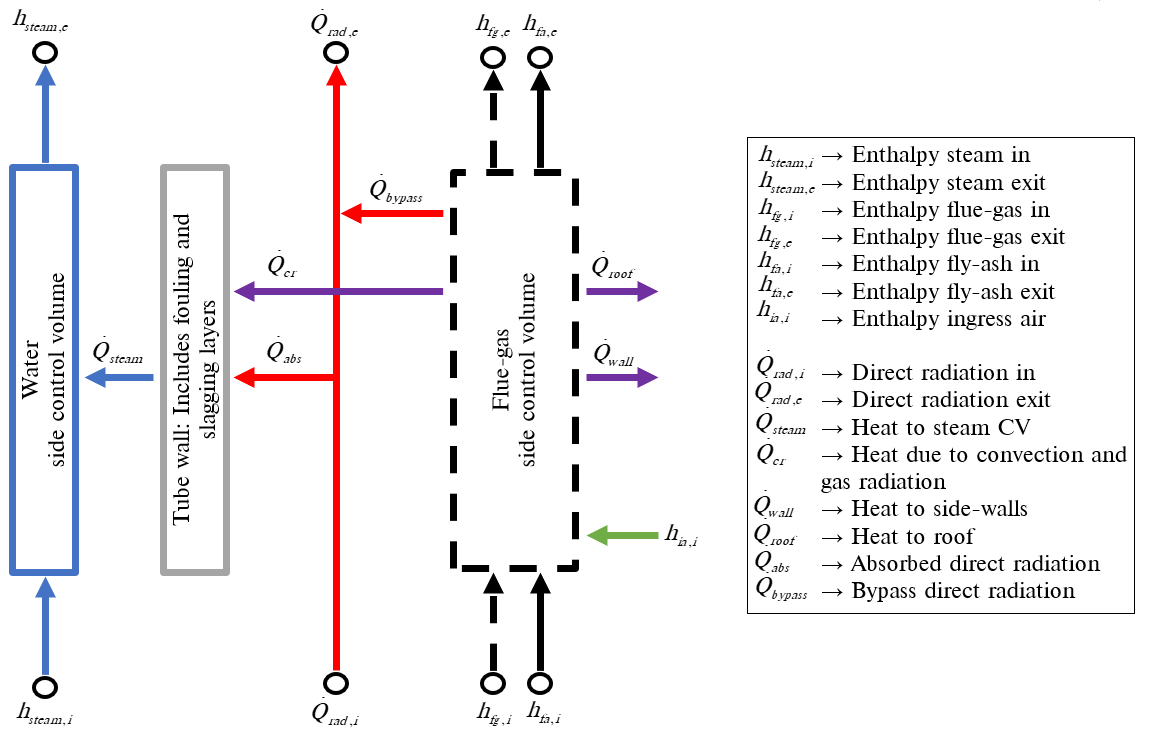
\includegraphics[scale=0.4]{HEAT_EXCHANGER_PROCESS_MODEL}}
\caption{Heat-exchanger component model}
\label{fig_heat_exchanger_model}
\end{figure*}

\subsection{Model inputs}
Table \ref{tbl_fuel} presents the coal characteristics utilized in the current study along with the higher heating value (HHV) of the fuel.\\

\begin{table}[h!]
\centering
\caption{Utility boiler fuel characteristics}
\vspace{2mm}
\label{tbl_fuel}
\begin{tabularx}{3.25in}{p{1.5in} p{0.8in} l}
\hline
\textbf{Fuel constituent} & \textbf{Fraction} & \textbf{Unit}\\
\hline
\textit{Ultimate analysis - (DAF)} & \textit{-} & \textit{-}\\
Carbon & $0.7753$ & $kg/kg_{fuel}$\\
Hydrogen & $0.0415$ & $kg/kg_{fuel}$\\
Nitrogen & $0.0181$ & $kg/kg_{fuel}$\\
Oxygen & $0.1474$ & $kg/kg_{fuel}$\\
Sulphur & $0.0175$ & $kg/kg_{fuel}$\\
\textit{Proximate analysis - (AR)} & \textit{-} & \textit{-}\\
Fixed carbon & $0.340$ & $kg/kg_{fuel}$\\
Volatile matter & $0.196$ & $kg/kg_{fuel}$\\
Ash & $0.4090$ & $kg/kg_{fuel}$\\
Moisture & $0.0550$ & $kg/kg_{fuel}$\\
\hline
\textbf{Energy content - (DAF)} & \textbf{Value} &\\
\hline
Higher heating value & $15070$ & $kJ/kg_{fuel}$\\
\hline
\vspace{0pt}
\end{tabularx}
\end{table}

For a boiler load 32\% MCR the current operational protocol is to use the bottom front and rear burner rows to meet the low-load demand during start-up.  For this study six cases are simulated with the following three burner firing configurations being investigated:
\begin{enumerate}
\item Bottom front and rear row burners are fired (Case 1 \& Case 4)
\item Middle front and rear row burners are fired (Case 2 \& Case 5)
\item Bottom front and middle rear row burners are fired (Case 3 \& Case 6)
\end{enumerate}
\begin{table}[h!]
\centering
\caption{Case 1 to 6 model inputs on a per burner basis.}
\label{tbl_case_inputs}
\vspace{2mm}
{\tabulinesep=1.2mm
\begin{tabularx}{3.25in}{p{1.4in} p{0.75in} l}
\hline
Active burners & \textbf{Cases 1 - 3} & \textbf{Cases 4 - 6}\\
\hline
\textbf{Fuel flowrate} [$kg/s$]&3.14  &3.14\\
\textbf{PA flowrate} [$kg/s$]&4.95  &4.95\\
\textbf{SA flowrate} [$kg/s$]&14.85  &14.85\\
\hline
Non firing burners &  & \\
\hline
\textbf{SA flowrate} [$kg/s$]&5.0  &2.5\\
\hline
Input air temperatures& &\\
\hline
\textbf{PA} [$K$]&373  &373\\
\textbf{SA} [$K$]&520  &510\\
\hline
\textbf{Excess air coefficients} & \highlight{1.37} & \highlight{1.32}\\
\hline

\end{tabularx}}
\vspace{0pt}
\end{table}

A secondary air flow rate of 5 [$kg/s$] is typically fed through the non-firing burners, to ensure sufficient cooling of the burner and mixing of fuel and air in the combustion chamber,\hl{ with this being executed cases 1, 2 and 3}. The result is a high air-fuel ratio in the furnace, which leads to higher dry gas losses. To lower this loss, this study will investigate the effect of reducing the air-fuel ratio by lowering the non-firing burner SA flowrate from 5 to 2.5 [$kg/s$], \hl{with this permutation being executed in cases 3, 4 and 6}. Two permutations of the SA flowrate, at the non-firing burners, are used for each of the firing configurations mentioned above. Table \ref{tbl_case_inputs} shows the input conditions for Cases 1 to 6. This data was obtained via conventional boiler mass and energy balance calculations.

\subsection{Numerical solution strategy}\label{sec_num_sol}
The CFD simulations were performed using ANSYS Fluent v19.5\textsuperscript{\textregistered} pressure-based solver. The pressure-momentum coupling utilised the SIMPLE method. Second-order upwinding was used to discretize the momentum, energy and species equations, whereas PRESTO! was used to discretize the pressure equation. The scalar field equations used a second-order upwind scheme.\\

The spatial discretization for all fields (except pressure) was set to first-order upwind for the first 1000 iterations to ensure a stable solution, after which the discretization order was increased to the above mentioned criteria. For all cases the maximum mass imbalance was 0.024 [$kg/s$] for a total gas flowrate of 190 [$kg/s$], and a heat imbalance of 1770 [$kW$] for a total heat input of 283 [$MW$]. The remaining fields were solved till convergence.\\

\hl{A numerical mesh consisting of roughly 6 million cells was used for the CFD simulations of this current study. To ensure that the results are grid size independent, simulations were also performed for mesh sizes of 3.5 million and 10 million cells during the validation study of Section} \ref{sec_model_valid}.

\section{Results \& discussion}
\subsection{Model validation}\label{sec_model_valid}
The validation of the proposed model was conducted for three steady-state MCR loads of 100\%, 80\% and 60\% respectively. Actual plant measurements were used to calculate the thermal heat loads of the three heat exchangers, namely the furnace, platen and final SH, to quantify the accuracy. The model inputs and boundary conditions can be obtained from the study conducted by Laubscher and Rousseau \cite{Laubscher2019b}, where using the same boiler of the present study, they evaluated the thermal performance of the heat exchanging components at full and reduced boiler loads.\\

Figure \ref{fig_heat_valid} shows that the calculated overall heat loads are in good agreement with the measured values where the model results are within the associated uncertainty range in all but one case. The simulation systematically under predicts the furnace heat loads, with a maximum percentage error of 2\%, while predominating overpredicting the platen SH loads, with a maximum percentage error of 7\%.\\

The CFD model was further validated by comparing the $CO_{ppm}$ and $X_{O_{2}}$ measurements against the CFD results. The probe measurements were taken at a furnace height of 37.5 [$m$] near the center of the boiler during full load (100\% MCR) operating conditions. The probe is inserted from the side walls to a depth of 4.5 [$m$], and measurements were taken every 0.5 [$m$].\\

\begin{figure*}[h]
\centerline{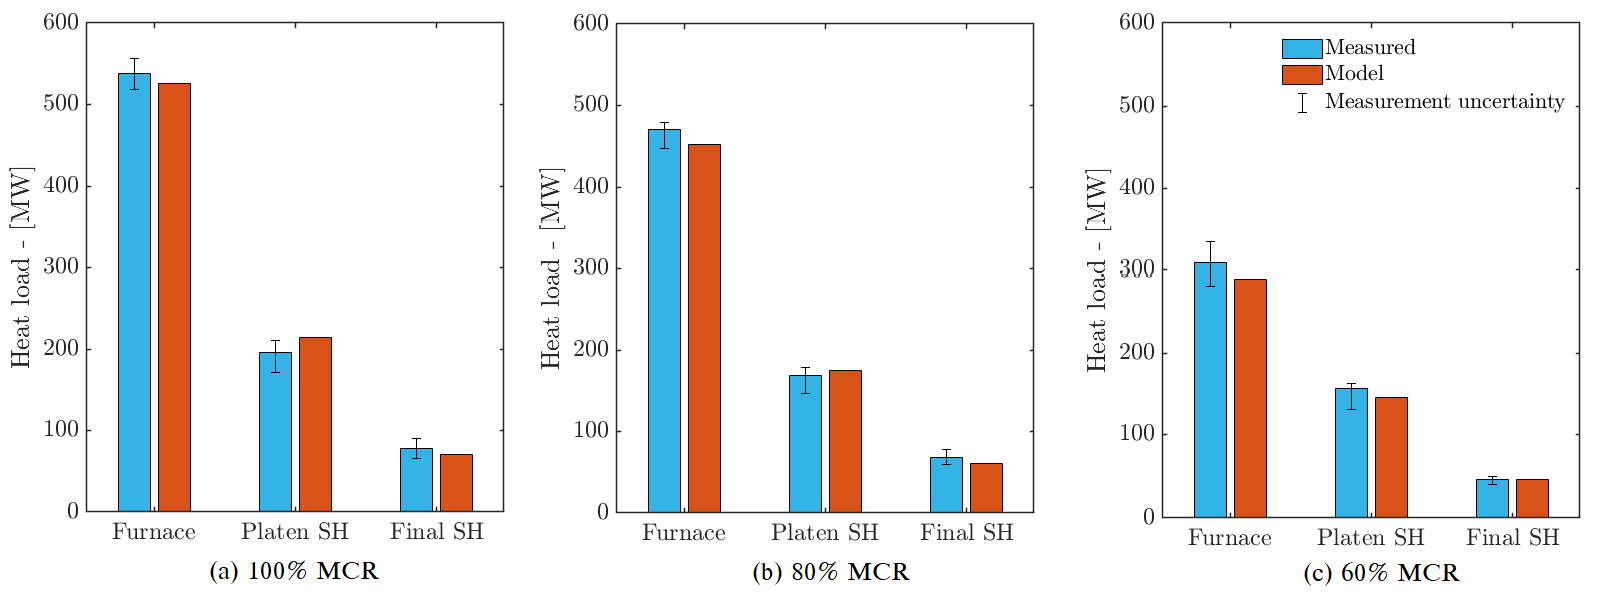
\includegraphics[scale = 0.4]{VALIDATION}}
\caption{Comparison of experimentally calculated and model heat loads for the furnace, platen SH and final SH}
\label{fig_heat_valid}
\end{figure*}
\begin{figure}[h!]
\centering
\subfigure[]{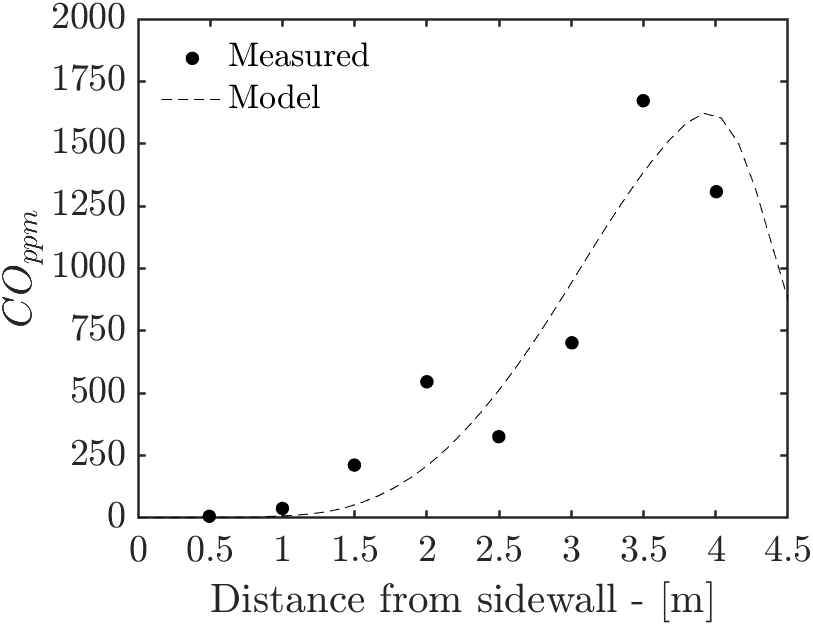
\includegraphics[width = 3.25in, height =5cm ]{COPPM_VALID}}
\hspace{5mm}
\subfigure[]{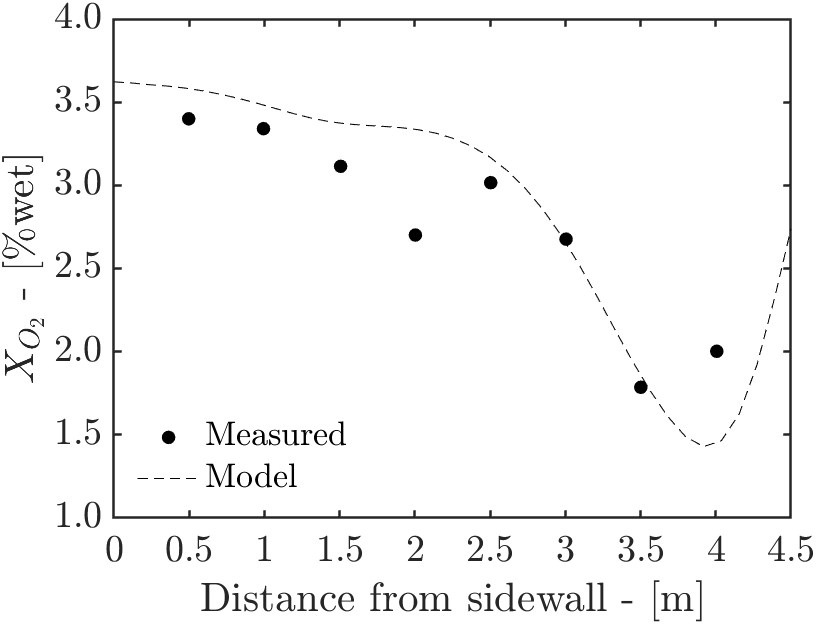
\includegraphics[width = 3.25in, height =5cm ]{XO2_VALID}}
\caption{Measured and predicted $CO_{ppm}$ (a) and $X_{O_{2}}$ (b) concentrations}
\label{fig_probe_valid}
\end{figure}
Figure \ref{fig_probe_valid} shows the averaged measurement values compared to the CFD predictions. It can be seen that the CFD model can resolve the $CO_{ppm}$ and $X_{O_{2}}$ concentrations at the given probe location with sufficient accuracy.

\subsection{Simulation results for various burner firing arrangements at 32\% MCR }
The temperature and velocity profiles for the various firing arrangements are shown in Fig. \ref{fig_cfd_temp} and Fig. \ref{fig_cfd_velo} respectively. With the middle burner rows firing (Cases 2 and 5) a substantial cold region is formed in the lower half the furnace, resulting in the lowest heat uptake. This is further exacerbated when considering Tab. \ref{tbl_process_parameters} where it is illustrated that the mid-firing arrangements produce the lowest steam flow rates resulting in the lowest boiler efficiencies. The bottom firing arrangement (Cases 1 and 4) results in a high temperature zone located in the bottom half on the burner, while the mixed firing arrangement (Cases 3 and 6) results is an even distribution of high temperature gases across the furnace domain (Fig. \ref{fig_cfd_temp}). This leads to the highest steam generation rate in the furnace and boiler efficiency as shown in Tab. \ref{tbl_process_parameters}.\\

\begin{figure*}[h!]
\centering
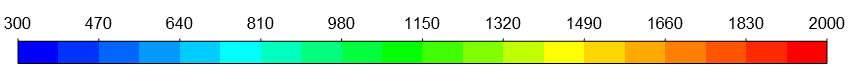
\includegraphics[width = 5in]{TEMP_KEY} [$K$]\\
\subfigure[Case 1]{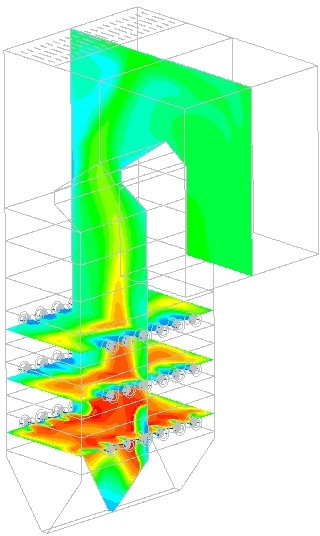
\includegraphics[width=0.25\textwidth]{BOT_TEMP}}
\subfigure[Case 2]{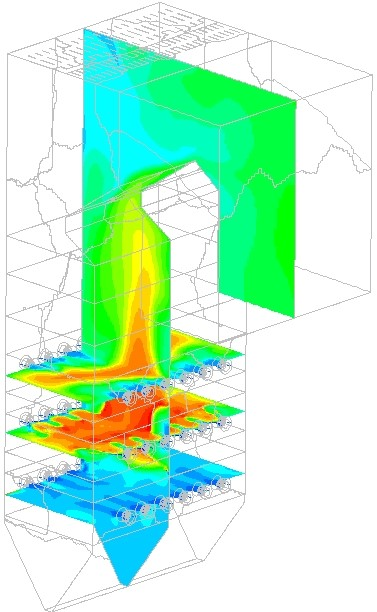
\includegraphics[width=0.25\textwidth]{MID_TEMP}}
\subfigure[Case 3]{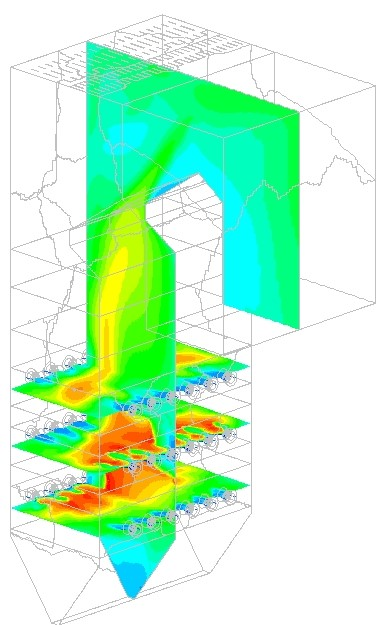
\includegraphics[width=0.25\textwidth]{FBRM_TEMP}}\\
\subfigure[Case 4]{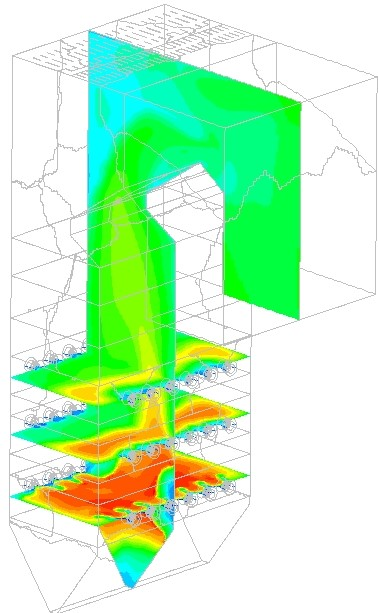
\includegraphics[width=0.25\textwidth]{BOT05_TEMP}}
\subfigure[Case 5]{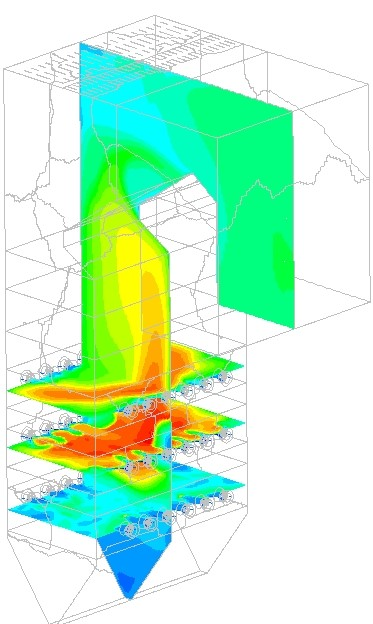
\includegraphics[width=0.25\textwidth]{MID05_TEMP}}
\subfigure[Case 6]{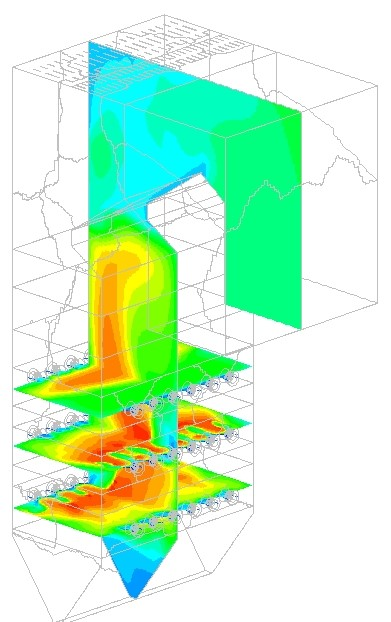
\includegraphics[width=0.25\textwidth]{FBRM05_TEMP}}
\caption{Temperature fields for Cases 1 through 6 [(a)-(f)]}
\label{fig_cfd_temp}
\end{figure*}

\begin{figure*}[h!]
\centering
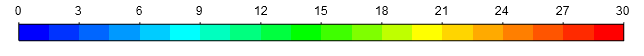
\includegraphics[width = 5in]{VEL_KEY} [$m/s$]\\
\subfigure[Case 1]{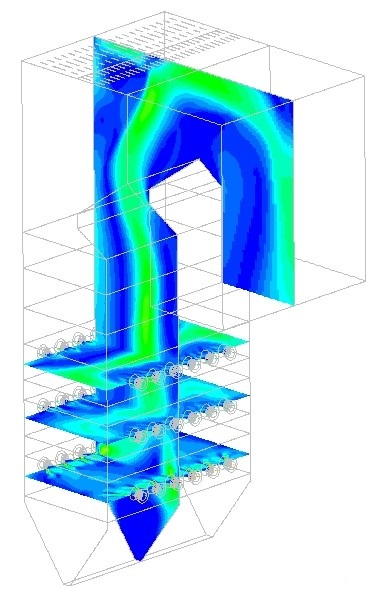
\includegraphics[width=0.25\textwidth]{BOT_VEL}}
\subfigure[Case 2]{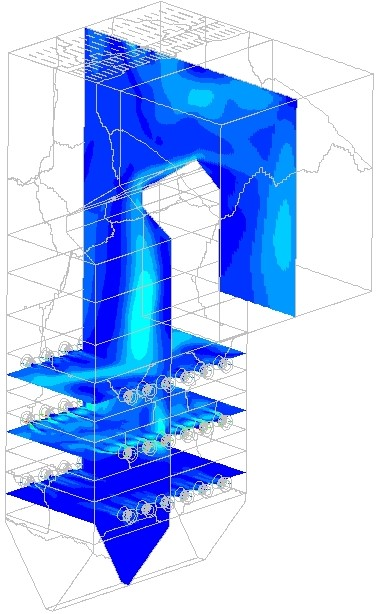
\includegraphics[width=0.25\textwidth]{MID_VEL}}
\subfigure[Case 3]{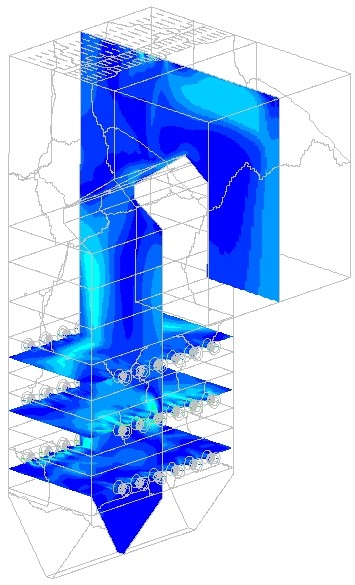
\includegraphics[width=0.25\textwidth]{FBRM_VEL}}\\
\subfigure[Case 4]{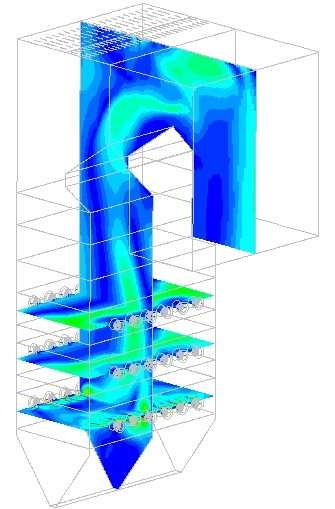
\includegraphics[width=0.25\textwidth]{BOT05_VEL}}
\subfigure[Case 5]{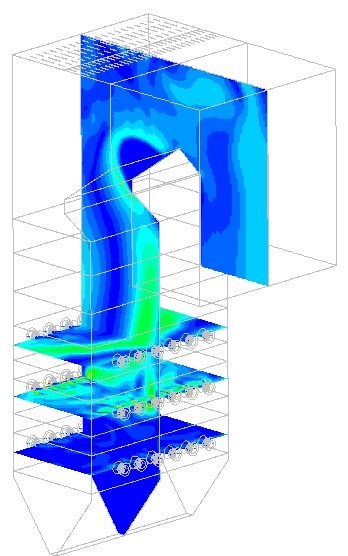
\includegraphics[width=0.25\textwidth]{MID05_VEL}}
\subfigure[Case 6]{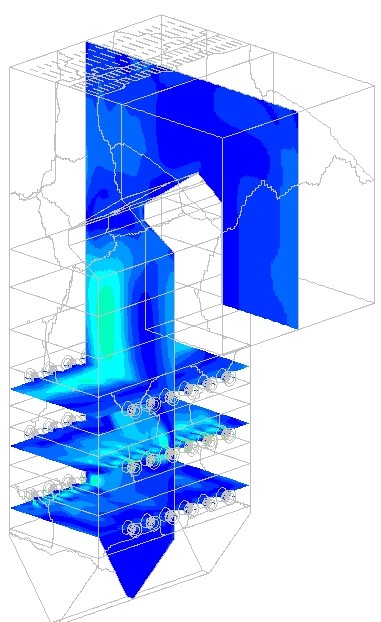
\includegraphics[width=0.25\textwidth]{FBRM05_VEL}}
\caption{Velocity fields for Cases 1 through 6 [(a)-(f)]}
\label{fig_cfd_velo}
\end{figure*}
\begin{table}[h!]
\centering
\caption{Furnace exit conditions and SH wall temperatures}
\vspace{2mm}
\begin{tabularx}{\linewidth}{p{1in} XXXXXX}
\hline
&\multicolumn{6}{c}{Cases}\\
 & \textbf{1} & \textbf{2} & \textbf{3}& \textbf{4}&\textbf{5}&\textbf{6}\\
\hline
\multicolumn{7}{l}{\textit{Furnace exit}}\\
\textbf{Exit temperature} [$K$] & 1168 & 1230 & 1215 & 1208 & 1306 & 1298\\
\textbf{Unburnt carbon} [$(\times 10^{-3})\,\%$] & 1.83 & 1.94 & 1.54 & 1.81 & 1.89 & 1.62\\
\multicolumn{7}{l}{\textit{Platen SH}}\\
\textbf{Max wall temperature} [$^{\circ}C$]  &477 & 492 & 481  & 480 & 493 & 490\\
\textbf{Mean wall temperature} [$^{\circ}C$] &439 & 453 & 446 & 454 & 442 & 451\\
\multicolumn{7}{l}{\textit{Final SH}}\\
\textbf{Max wall temperature} [$^{\circ}C$]  & 602 & 624 & 608 & 595 & 626 & 612\\
\textbf{Mean wall temperature} [$^{\circ}C$] & 520 & 523 & 517 & 512 & 520 & 511\\
\hline
\label{tbl_cfd_results}
\end{tabularx}
\end{table}
\newpage
Figure \ref{fig_cfd_heat_flux} illustrates the heat flux profiles for the simulated cases. Both cases 1 and 4 highlight high heat flux zones near the burner inlets which, in the presence of high temperatures and incomplete combustion near these regions, can lead to high-temperature corrosion \cite{ugum2019}. An even distribution of heat fluxes is seen in Cases 3 and 6 with minimal localised heat flux concentrations being observed. Cases 2 and 5 show that most of the heat is absorbed in the upper half of the boiler with Case 5 showing a higher heat flux on the rear wall. This could be due the use of a lower SA flowrate leading to higher velocity profiles developing closer to the rear wall, as seen in Fig. \ref{fig_cfd_velo}. \hl{With this in mind} a lower SA flowrate, in general leads to hot gases and velocity profiles impinging closer to the furnace walls, which can be seen in Cases 4, 5 and 6 of Fig. \ref{fig_cfd_temp} and Fig.\ref{fig_cfd_velo} respectively. With high gas temperatures and high velocity impingement, Cases 4, 5 and 6 (of Fig. \ref{fig_cfd_heat_flux}) experience concentrated heat fluxes around the burner inlets in comparison to corresponding Cases 1, 2 and 3.\\

\begin{figure*}[h!]
\centering
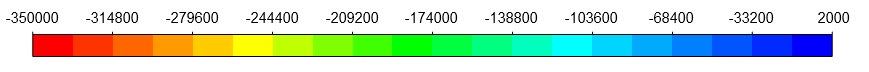
\includegraphics[width = 5in]{HEATFLUX_KEY} [$W/m^2$]\\
\subfigure[Case 1]{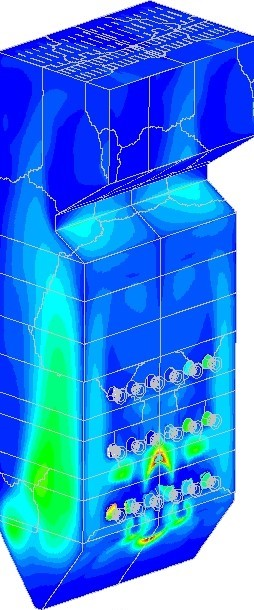
\includegraphics[width=0.18\textwidth]{BOT_HEATFLUX}}
\hspace{10mm}
\subfigure[Case 2]{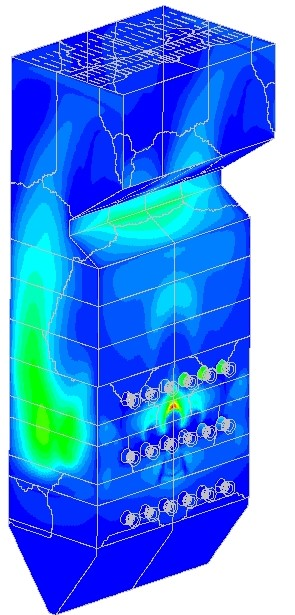
\includegraphics[width=0.2\textwidth]{MID_HEATFLUX}}
\hspace{10mm}
\subfigure[Case 3]{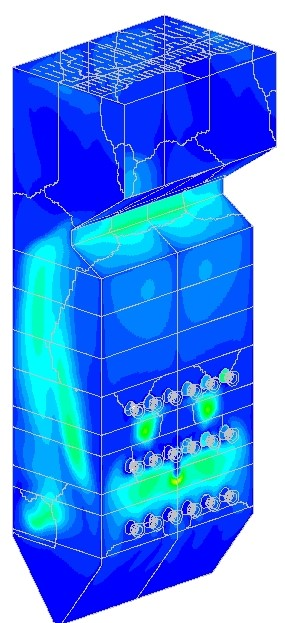
\includegraphics[width=0.2\textwidth]{FBRM_HEATFLUX}}\\
\subfigure[Case 4]{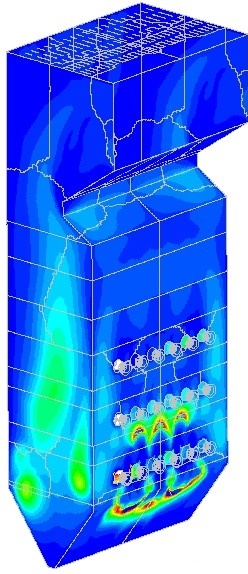
\includegraphics[width=0.18\textwidth]{BOT05_HEATFLUX}}
\hspace{10mm}
\subfigure[Case 5]{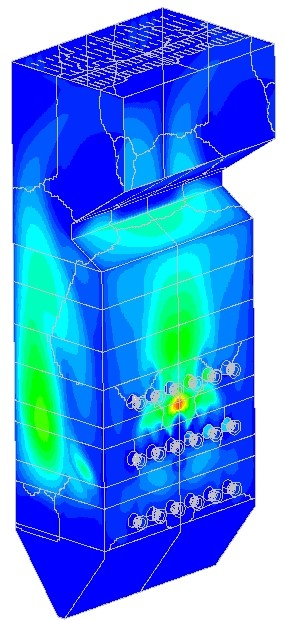
\includegraphics[width=0.2\textwidth]{MID05_HEATFLUX}}
\hspace{10mm}
\subfigure[Case 6]{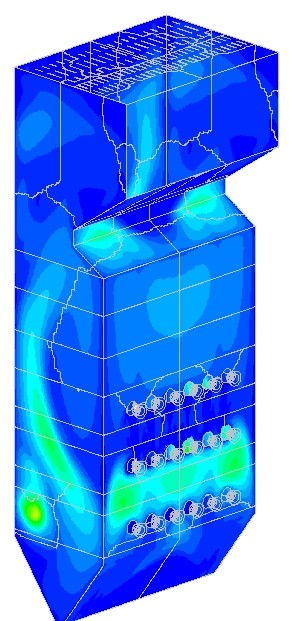
\includegraphics[width=0.2\textwidth]{FBRM05_HEATFLUX}}
\caption{Heat fluxes profiles for Cases 1 through 6 [(a)-(f)]}
\label{fig_cfd_heat_flux}
\end{figure*}
\newpage
\hl{The works of Dugum et al}\cite{ugum2019}, highlights the issue of high-temperature corrosion caused by significant levels of $CO$ ($X_{CO}$ 0.01 - 0.1) and no-free $O_2$ near regions of high wall temperatures. For low-load operation this phenomenon becomes important to avoid since combustion instability can lead to these non-ideal circumstances. Figure \ref{fig_cfd_coppm} shows the $CO$ molar concentration in the domain located on an iso-surface set 1600 $[K]$. The figures generally highlight the location and distribution of the flame core for each case. Cases 1 and 4 illustrate the highest likelihood of high-temperature corrosion occurring near the furnace hopper, due to the high concentration and temperatures in that region.\\
\begin{figure*}[h!]
\centering
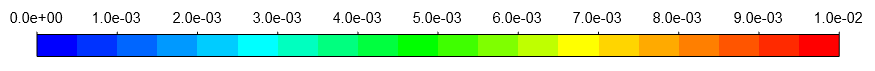
\includegraphics[width = 5in]{CO_MF_KEY} [$X_{CO}$]\\
\subfigure[Case 1]{	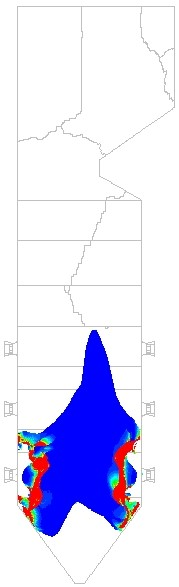
\includegraphics[width=0.16\textwidth, height = 7cm]{BOT_ISO_COPPM_F}
				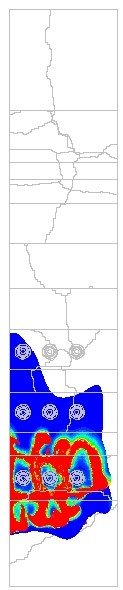
\includegraphics[height = 7cm]{BOT_ISO_COPPM_S}}
\hspace{5mm}
\subfigure[Case 2]{	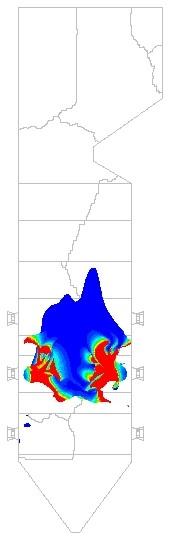
\includegraphics[width=0.16\textwidth, height = 7cm]{MID_ISO_COPPM_F}
				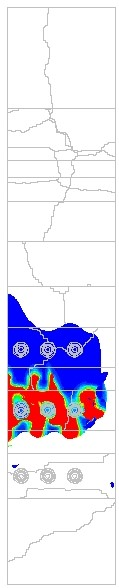
\includegraphics[height = 7cm]{MID_ISO_COPPM_S}}
\hspace{5mm}
\subfigure[Case 3]{	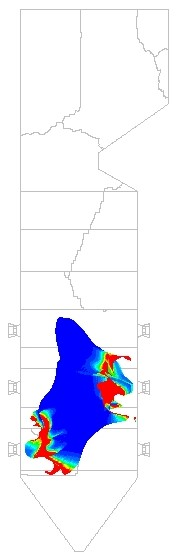
\includegraphics[width=0.16\textwidth, height = 7cm]{FBRM_ISO_COPPM_F}
				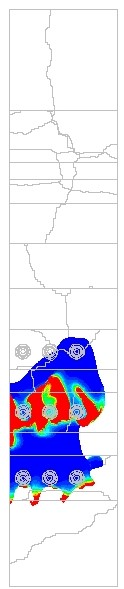
\includegraphics[height = 7cm]{FBRM_ISO_COPPM_S}}\\
\subfigure[Case 4]{	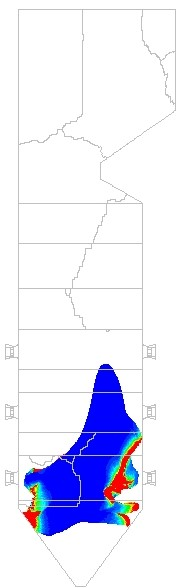
\includegraphics[width=0.16\textwidth, height = 7cm]{BOT05_ISO_COPPM_F}
				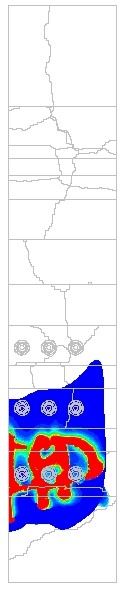
\includegraphics[height = 7cm]{BOT05_ISO_COPPM_S}}
\hspace{5mm}
\subfigure[Case 5]{	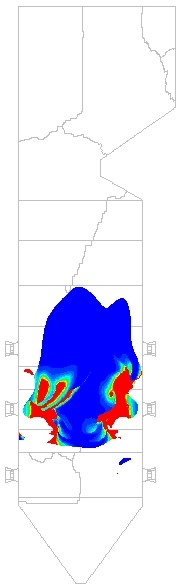
\includegraphics[width=0.16\textwidth, height = 7cm]{MID05_ISO_COPPM_F}
				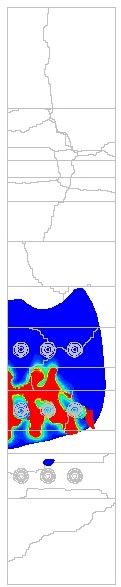
\includegraphics[height = 7cm]{MID05_ISO_COPPM_S}}
\hspace{5mm}
\subfigure[Case 6]{	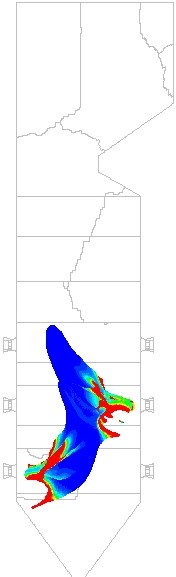
\includegraphics[width=0.16\textwidth, height = 7cm]{FBRM05_ISO_COPPM_F}
				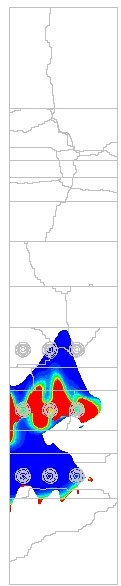
\includegraphics[height = 7cm]{FBRM05_ISO_COPPM_S}}
\caption{CO molar fraction ($X_{CO}$) concentrations for 
Cases 1 through 6 [(a)-(f)] on a temperature iso-surface of 1600 [K]}
\label{fig_cfd_coppm}
\end{figure*}

Investigating the combustion stability for all the cases, the symmetry and offset vertical probe plots (as highlighted in Fig. \ref{fig_geometry}) are given in Fig. \ref{fig_cfd_probe}. Cases 2 and 5 illustrates the highest $X_{O_{2}}$ concentration in the lower half of the burner since there is minimal combustion occurring. The unburnt carbon content and exit flue-gas temperatures for each case are reported in Tab. \ref{tbl_cfd_results}. With the use of the middle burners (Cases 2 and 5) the highest exit temperature and unburnt carbon content is observed, since the flame core is located in the upper half of the furnace leading to the least possibility of complete combustion due to the shorter residence time. Cases 3 and 6 exhibit the best characteristics with the least amount of unburnt carbon content being observed. It is important to note the effects of a lower SA mass flow rate has on the furnace exit conditions for non-firing burners, which generally leads to a hotter exit gas temperature as seen with Cases 4 to 6. \\

\begin{figure*}[h!]
\centering
\subfigure[Symmetry vertical plot]{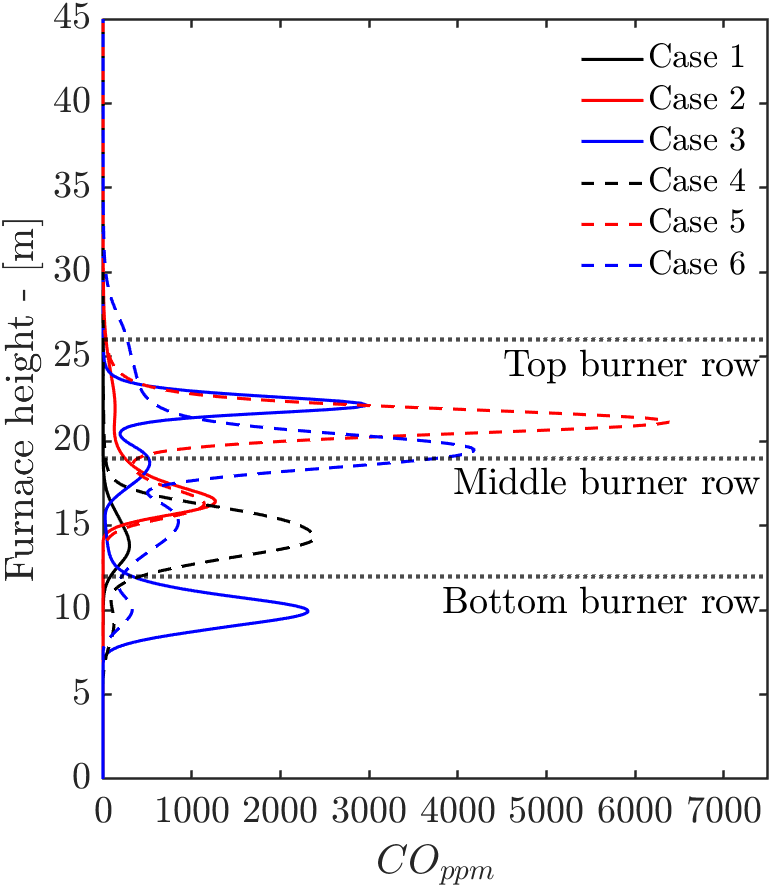
\includegraphics[scale = 0.45]{SYMMETRY_PROBE_COPPM}}
\hspace{5mm}
\subfigure[Offset vertical plot]{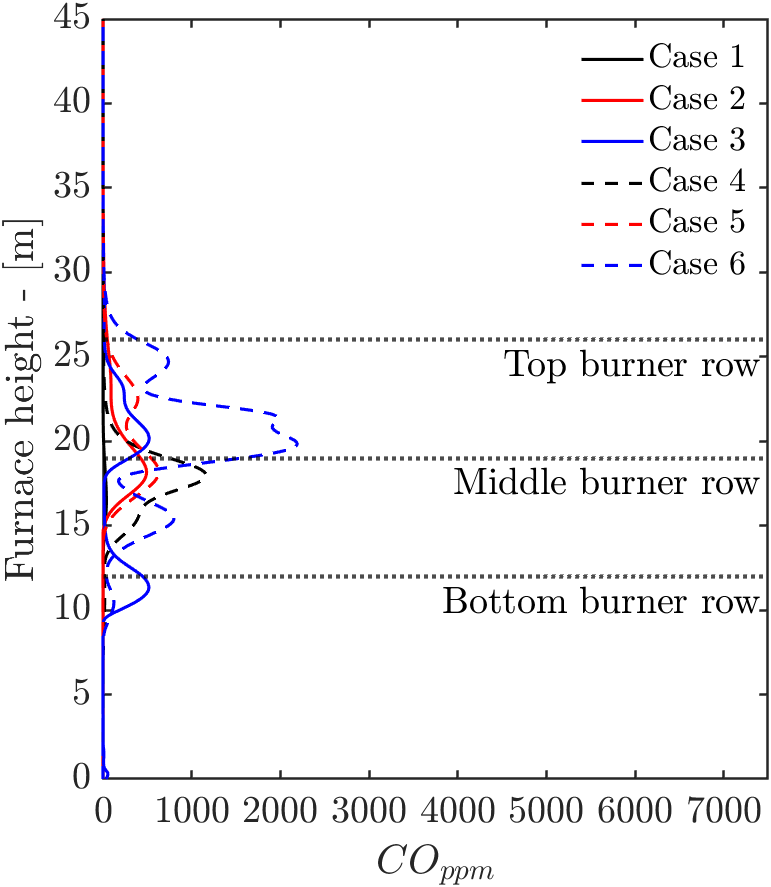
\includegraphics[scale = 0.45]{OFFSET_PROBE_COPPM}}
\hspace{5mm}
\subfigure[Symmetry vertical plot]{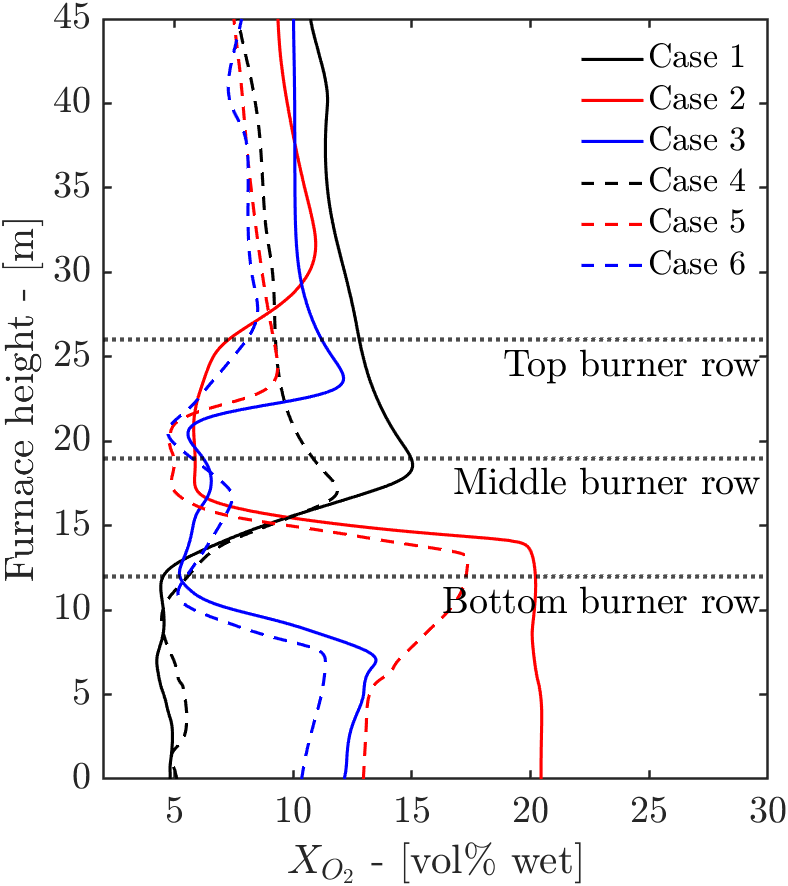
\includegraphics[scale = 0.45]{SYMMETRY_PROBE_XO2}}
\hspace{5mm}
\subfigure[Offset vertical plot]{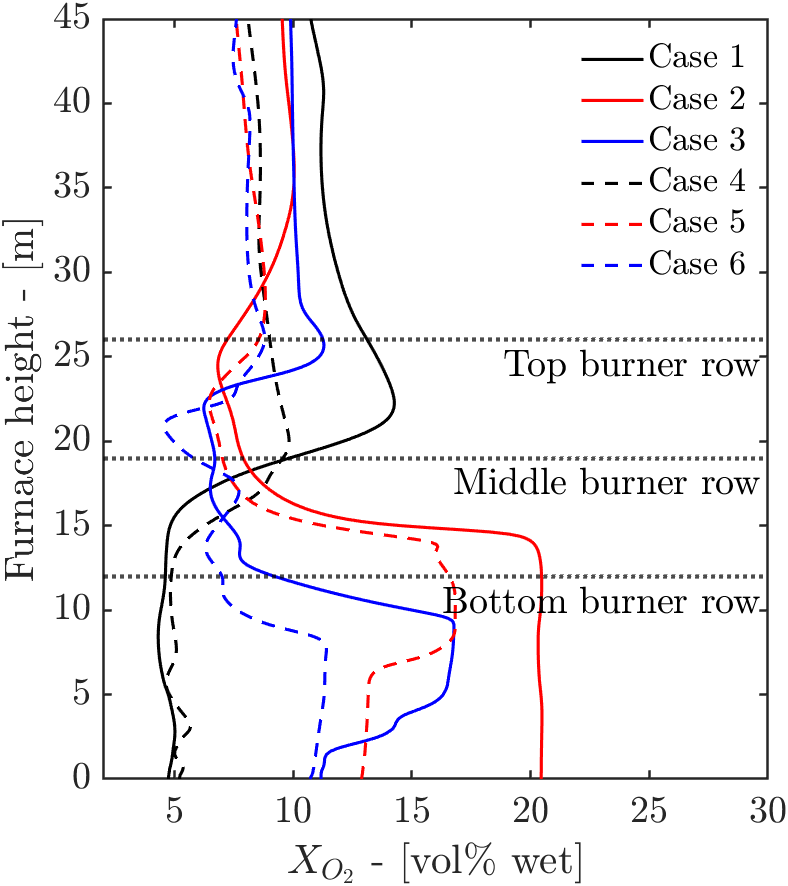
\includegraphics[scale = 0.45]{OFFSET_PROBE_XO2}}
\caption{$CO_{PPM}$ [(a) and (b)] and $X_{O_{2}}$ [(c) and (d)] line plots on symmetry and offset vertical probe lines}
\label{fig_cfd_probe}
\end{figure*}

The external tube metal temperatures, shown in Tab. \ref{tbl_cfd_results} were calculated using Eqn. \ref{eqn_t_wall}, which takes into account the temperature drop due to the ash deposit present on platen and final SH. Fouling thermal resistances of 0.0067 and 0.015 [$m^2K/W$] were used for the platen and final SH respectively.
\begin{equation}\label{eqn_t_wall}
T_{metal} = T_{wall} - \left(\frac{\dot{q}_{SH}t_{ASH}}{\lambda_{ASH}}\right)
\end{equation}

For the platen and final SH the maximum surface temperature are observed for Cases 2 and 5. For comparison, at 100\% MCR load the maximum and mean temperatures reported for the platen and final SH are 500 \& 446 $[^\circ C]$ and 623 \& 531 $[^\circ C]$ respectively, with the final SH operating in the materials creep range \cite{Laubscher2019b}. Thus, continued operation using the firing arrangement of Cases 2 and 5, could lead to SH failure.\\
\newpage
Using the process model of Fig. \ref{fig_flownex} and the results of the CFD simulations the important process control parameters were determined. Table \ref{tbl_process_parameters} summarizes the results with the highest boiler efficiencies observed for Cases 3 and 6. With a lower SA flowrate Cases 4 to 6 exhibit a higher boiler efficiency due to the decrease in dry gas losses, when compared to Cases 1 to 3. All cases exhibit adequate control of the main steam exit temperature by use of ATT1 and ATT2. The exit temperature of the reheaters, for all Cases, are determined to within the 20 [$^\circ C$] tolerance for the intermediate turbine inlet conditions, as stipulated in the design C-schedules for the plant. However, with the lack of ATT-RH control, a sudden decrease in steam generation can lead to RH overheating and possible RH failure. Considering all of the above, Cases 3 and 6 are seen as the best firing arrangements for continuous low-load operation at a load of 32\% MCR.\\

\begin{table}[h!]
\centering
\caption{Process model control parameters}
\vspace{2mm}
\begin{tabularx}{\linewidth}{p{1in} XXXXXX}
\hline
&\multicolumn{6}{c}{Cases}\\
 & \textbf{1} & \textbf{2} & \textbf{3}& \textbf{4}&\textbf{5}&\textbf{6}\\
\hline
\textbf{Main steam flowrate} 	[$kg/s$]		&175.8&172.9&180.5&180.2&179.1&184.1 \\
\textbf{Main steam exit temp} 	[$^{\circ}C$]	&535& 535 &535&535 &535& 535\\
\textbf{RH steam flow rate} 	[$kg/s$]		&158.2&155.6&162.5&162.2&161.2&165.6\\
\textbf{RH steam exit temp} 	[$^{\circ}C$]	&524&527&531&512&510&520\\
\textbf{Boiler efficiency} 		[$\%$]			&85.3&84.1&87.9	&87.2&85.9&89.1\\
\textbf{ATT1} 		[$kg/s$]					&10.4&16.9&13.9&7.9&5.5&10.9\\
\textbf{ATT2} 		[$kg/s$]					&1.7&3.8&4.2&3.8&3.6&4.2\\
\textbf{ATT-RH} 		[$kg/s$]				&0.0&0.0&0.0&0.0&0.0&0.0\\
\hline
\label{tbl_process_parameters}
\end{tabularx}
\end{table}

\begin{table}[h!]
\centering
\caption{Radiative heat transfer percentage for Cases 3 and 6}
\vspace{2mm}
{\tabulinesep=1.2mm
\begin{tabularx}{\linewidth}{p{0.4\linewidth} XX}
\hline
 &\textbf{Case 3}&\textbf{Case 6}\\
\hline
Furnace [\%] & 89.2 & 88.9\\
Platen SH (SH2) [\%] & 92.5& 93.4\\
Final SH (SH3) [\%] & 93.5& 94.0\\
RH2 [\%] & 47.6& 52.2\\
SH1 [\%] & 37.2& 40.7\\
RH1 [\%] & 18.7& 21.5\\
EC [\%] & 5.4& 6.5\\
\hline
\label{tbl_rad_conv}
\end{tabularx}}
\end{table}
\newpage
Table \ref{tbl_rad_conv} shows the radiative heat percentage of the total heat input into each heat-exchanger for Cases 3 and 6. It can be seen that heat transfer to the furnace and radiant SHs are dominated by radiation, with approximately $\pm$ 10\% being transferred via convection at low-load. Considering the convective pass heat exchangers (RH2 through to the EC, refer to Figure \ref{fig_flownex}) the convective heat transfer becomes more apparent as seen with the reduction in radiative heat transfer percentage. Case 6 involves less convective heat transfer due to the SA flowrate for non-firing burners. This will reduce the total amount of flue-gas flowing through the boiler, thereby reducing the convective heat transfer.
\newpage

\section{Conclusions}
The present study demonstrates the use of a coupled CFD/process model to study the effects of burner configuration at a boiler load of 32\% MCR. A validation case was first performed for the CFD model, which showed adequate results for heat fluxes to the walls, with a general tendency of the model to under-predict the heat fluxes to the furnace. The model also showed sufficient accuracy in determining the combustion characteristics at the 100 \% MCR load.\\ 

The subsequent analysis results show that using a burner arrangement that raises the position of the flame core (Cases 2 and 5) increases the exit flue-gas temperature and runs the risk of final SH failure due to overheating. This firing arrangement also results in a higher unburnt carbon percentage at the exit flue-gas stream and therefore the lowest boiler utilization efficiency. \\

Operation of the boiler using firing arrangements of Cases 1 and 4 also results in a lower boiler utilization efficiency and exit flue-gas temperature compared to Cases3 and 6. Higher $X_{CO}$ concentrations are observed near the bottom half of the furnace, along with high temperatures, which can lead to a high risk of fire side corrosion occurring at continuous low-load operation. \\

The mixed firing arrangements, of Cases 3 and 6, exhibit the best boiler utilization efficiencies. A 4.8\% decrease in unburnt carbon percentage is observed when operating using Case 3 in relation to Case 6. The predicted re-heater exit steam temperature of Case 3 is substantially closer to the desired temperature of 535 $[^\circ C]$, thus allowing for better control.\\
\newpage
Based on analyses of combustion stability, boiler efficiency and the safe operation of heat exchanger components, Case 3 is considered to be the best operational strategy at this low load for the boiler under investigation.


\newpage
%%%%%%%%%%%%%%%%%%%%%%%%%%%%%%%%%%%%%%%%%%%%%%%%%%%%%%%%%%%%%%%%%%%%%%
\begin{acknowledgment}
The authors would like to thank the Eskom EPPEI program for financially supporting the present study and acknowledge the computational resources provided by the Centre for High Performance Computing (CHPC), South Africa.
\end{acknowledgment}

%%%%%%%%%%%%%%%%%%%%%%%%%%%%%%%%%%%%%%%%%%%%%%%%%%%%%%%%%%%%%%%%%%%%%%
% The bibliography is stored in an external database file
% in the BibTeX format (file_name.bib).  The bibliography is
% created by the following command and it will appear in this
% position in the document. You may, of course, create your
% own bibliography by using thebibliography environment as in
%
% \begin{thebibliography}{12}
% ...
% \bibitem{itemreference} D. E. Knudsen.
% {\em 1966 World Bnus Almanac.}
% {Permafrost Press, Novosibirsk.}
% ...
% \end{thebibliography}

% Here's where you specify the bibliography style file.
% The full file name for the bibliography style file 
% used for an ASME paper is asmems4.bst.
\bibliographystyle{asmems4}

% Here's where you specify the bibliography database file.
% The full file name of the bibliography database for this
% article is asme2e.bib. The name for your database is up
% to you.
\newpage
\bibliography{PAPER1_LOW_LOAD}


\end{document}
